\documentclass{beamer}

\usepackage{subfigure}

\title{....}
\author{Qiayuan Liao\inst{1}}
\date{June 16, 2019}

\institute[] % (optional)
{
  \inst{1}
  liaoqiayuan@gmail.com
}

\begin{document}

\begin{frame}
  \titlepage
  \rightline{Power by \LaTeX}
\end{frame}

\begin{frame}
  \frametitle{Outline}
  \tableofcontents
\end{frame}

\section{Manipulation}

\begin{frame}
  \frametitle{Manipulation}
  \vspace{-2.0cm}
  \begin{columns}
    \column{0.5\textwidth}
    PD + feedforward control of ball screw linear actuator:
    \begin{itemize}
      \item Large Load
      \item High Speed Requirement
    \end{itemize}

    \column{0.4\textwidth}
    \begin{figure}
      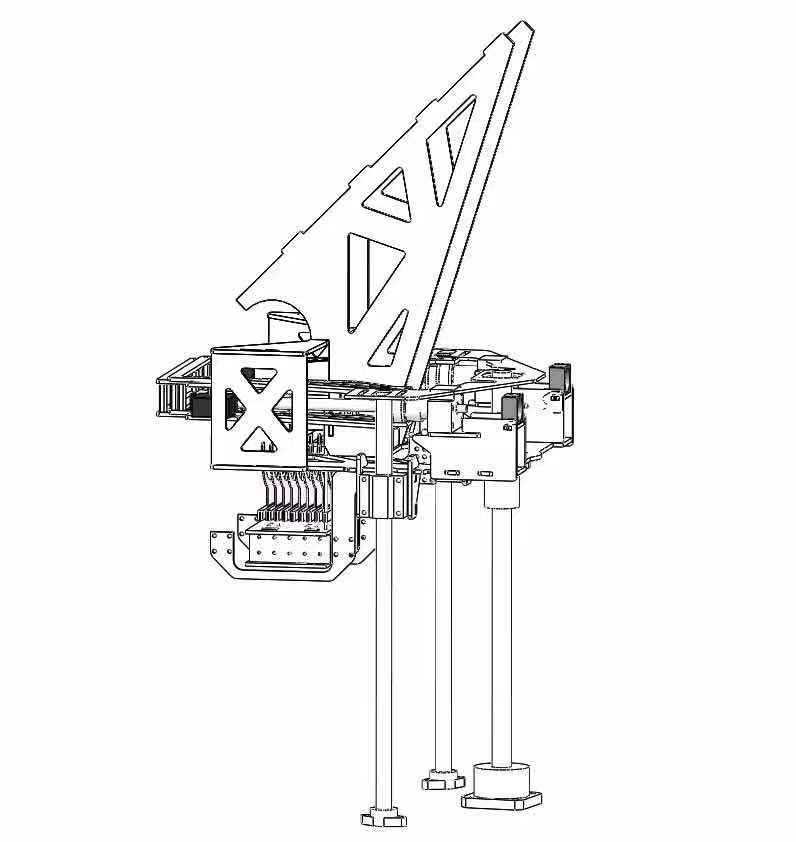
\includegraphics[width = 0.8\textwidth]{fig/screw.jpg}
      \caption{Basll screw actuator and its load}
    \end{figure}
  \end{columns}
  \begin{equation}
    \tau = k_p(z_{ref}-z_{now})+k_d(\dot{z}_{ref}-\dot{z}_{now})+ \frac{mgh}{2\pi \eta}
  \end{equation}
  where $h$ is feed screw lead, $\eta$ is positive efficiency of feed screw
\end{frame}

\section{locomotion}
\subsection{Kinematic}
\begin{frame}
\frametitle{Kinematic}
\begin{columns}
\column{0.65\textwidth}
  \begin{equation}
  ^W\mathbf{R}_R =
    \begin{bmatrix}
      cos(\theta) & -sin(\theta) & 0 \\
      sin(\theta) &  cos(\theta) & 0 \\
      0 &  0 & 1 \\
    \end{bmatrix}
  \end{equation}
  \begin{equation}
    ^W\mathbf{\xi}_R =
      \begin{bmatrix}
        cos(\theta) & -sin(\theta) & 0 & x\\
        sin(\theta) &  cos(\theta) & 0 & y\\
        0 & 0 & 1 & 0 \\
        0 & 0 & 0 & 1 \\
      \end{bmatrix}
  \end{equation}
  \column{0.4\textwidth}

  \begin{figure}
    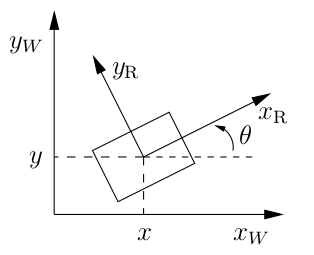
\includegraphics[width = \textwidth]{fig/pose.png}
    \caption{Definition of pose $\textbf{x} = (x, y, \theta)^T$, word and robot frame \cite{Roehrig2017@motion}}
  \end{figure}
  \end{columns}
\end{frame}

\subsection{Dynamics}
\begin{frame}
  \frametitle{Dynamics}
  State Space\cite{conceicao2010predictive}:
  \begin{equation}
  \mathbf{\dot x} = \mathbf{Ax}+\mathbf{Bu}
  \end{equation}
  where:
  \begin{eqnarray*}
    \mathbf{x} =
    \begin{bmatrix}
      x& y &\theta &\dot x& \dot y& \dot \theta
      \label{eqa:state}
    \end{bmatrix}^T
    \mathbf{u} =
    \begin{bmatrix}
      u_1& u_2& u_3& u_4
    \end{bmatrix}^T
  \end{eqnarray*}
  \begin{eqnarray*}
    \mathbf{A} =
    \begin{bmatrix}
      \textbf{0}_3 & \textbf{1}_3\\
      \textbf{0}_3 & \textbf{0}_3\\
    \end{bmatrix}
    \mathbf{B} =
    \begin{bmatrix}
      0 & 0 & 0 & 0\\
      0 & 0 & 0 & 0\\
      0 & 0 & 0 & 0\\
      \frac{\sqrt{2}}{M}& -\frac{\sqrt{2}}{M}& -\frac{\sqrt{2}}{M}& \frac{\sqrt{2}}{M}\\
      \frac{\sqrt{2}}{M}& \frac{\sqrt{2}}{M}& -\frac{\sqrt{2}}{M}& -\frac{\sqrt{2}}{M}\\
      l\cos(\frac{\pi}{4}-\alpha)/I_{zz}& \cdots &\cdots &l\cos(\frac{\pi}{4}-\alpha)/I_{zz}\\
    \end{bmatrix}\\
  \end{eqnarray*}

\end{frame}

\subsection{Path Planning}
\begin{frame}
\frametitle{Path Planning}
\begin{itemize}
  \item Gobal Planning
  \item Local Planning
  \item Cublic Spline
\end{itemize}
get: $\textbf{x}_{ref} = \begin{bmatrix}
  x_{ref}& y_{ref}& \theta_{ref}
\end{bmatrix}^T$
and $^W\mathbf{R}_{ref}$
\end{frame}

\subsection{Control}
\begin{frame}
  \frametitle{Control}
  \begin{itemize}
    \item PID Speed Control
    \item P Postion Control (0.5m/s)
    \item Line Following Control (1.2m/s)
    \item Omnidirectional Following Control (2.0m/s)
    \item Model Predictive Control
  \end{itemize}
\end{frame}
\begin{frame}
  \frametitle{Controller}
  Simple P Control:\\
  \begin{equation}
    ^R\mathbf{v} =^W\mathbf{R}_R^T \mathbf{K}_p(\textbf{x}_{now}-\textbf{x}_{ref})
  \end{equation}
  Line Following Control:\\
  \begin{equation}
    ^R\mathbf{v} =
    \begin{bmatrix}
    k_{maxSpeed}(1-\frac{\theta_{ref}-\theta_{now}}{k_{maxAngle}})& 0& k_p(\theta_{ref}-\theta_{now})
    \end{bmatrix}^T
  \end{equation}
  Omnidirectional Following Control:\\
  \begin{equation}
    ^R\mathbf{v} = ^W\mathbf{R}_{ref}\begin{bmatrix}
      k_{maxSpeed}\\0\\0
    \end{bmatrix}
  \end{equation}
\end{frame}



\subsection{Model Predictive Control}
\begin{frame}
  \frametitle{Model Predictive Control: Overview}
  \begin{figure}
    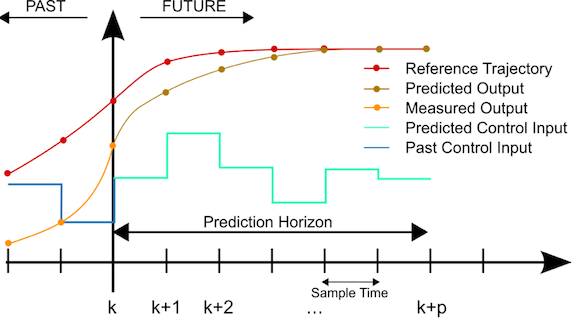
\includegraphics[width = 0.7\textwidth]{fig/MPC.png}
    \caption{MPC Overview}
  \end{figure}
  \vspace{-0.5cm}
  \begin{itemize}
    \item Handles multivariable interactions
    \item Handles input and output constraints
    \item Can push the plants to their limits of performance
  \end{itemize}
\end{frame}

\begin{frame}
  \frametitle{MPC: Theory}
  for each $t = k$, solve the optimization problem:
  \small
  \begin{eqnarray}
    l(x(i),u(i)) &=& \sum\limits_{i = 1}^N(x(k+i))-x_{ref}(k+i))^T\mathbf{Q}(x(k+i))-x_{ref}(k+i)) \nonumber \\
    &+&\sum\limits_{i = 0}^{N-1}(u(k+i))-u_{ref}(k+i))^T\mathbf{R}(u(k+i))-u_{ref}(k+i)) \nonumber
\end{eqnarray}
\vspace{-0.5cm}
\begin{alignat}{2}
    \min_{u,x} \quad &\sum\limits_{i=1}^N l(x(i),u(i)) \\
    \mbox{s.t.}\quad
    &x_{(k+1+i)}= \mathbf{\hat{A}}x(k+i) + \mathbf{\hat{B}}u(k+i), \nonumber\\
    &\quad \quad i=0,1,\dots,N-1,\label{con:model} \\
    &|u(k+i)| \leq u_{max}, \nonumber\\
    &\quad \quad i=0,1,\dots,N-1 \label{con:input}, \\
    &|x(k+i)| \leq x_{max}, \nonumber\label{con:state}\\
    &\quad \quad i=1,2,\dots,N,
\end{alignat}

\end{frame}

\begin{frame}
  \frametitle{MPC: Implement}
  Convert model(eqa(\ref{eqa:state})) from continuous to discrete time:
  \begin{equation}
  x_{(k+1)} = \hat{\mathbf{A}}x_{k}+\hat{\mathbf{B}}u_{k}
  \end{equation}
  Reformula to a QP(quadratic programming) problem:
  \begin{alignat}{2}
    \min_{\mathbf{U}} \quad & \frac{1}{2}\mathbf{U}^T\mathbf{HU}+\mathbf{U}^Tg \\
    \mbox{s.t.}\quad
    &l \leq \mathbf{CU} \leq u
  \end{alignat}
  \begin{itemize}
    \item Use Julia programming languages\cite{bezanson2017julia}
    \item Work with ROS
    \item Use OSQP\cite{osqp} solver
    \item Real time solving: 10000Hz maximum (actually only need 20~30Hz)
  \end{itemize}
\end{frame}

\begin{frame}[allowframebreaks]
  \frametitle{Reference}
  \begin{small}
  \bibliographystyle{plain}
  \bibliography{ref}
  \end{small}
\end{frame}


\end{document}
